\documentclass[conference]{IEEEtran}

\usepackage{cite}
\usepackage{pslatex} % -- times instead of computer modern, especially for the plain article class
\usepackage[colorlinks=false,bookmarks=false]{hyperref}
\usepackage{booktabs}
\usepackage{graphicx}
\usepackage{xcolor}
\usepackage{multirow}
\usepackage{comment}
%\usepackage{flushend} % even out the last page, but use only at the end when there is a bibliography

\newcommand{\code}[1]{{\small{\texttt{#1}}}}

% fatter TT font
\renewcommand*\ttdefault{txtt}
% another TT, suggested by Alex
% \usepackage{inconsolata}
% \usepackage[T1]{fontenc} % needed as well?

\usepackage{listings}

%\newcommand{\todo}[1]{{\emph{TODO: #1}}}
\newcommand{\todo}[1]{{\color{olive} TODO: #1}}
\newcommand{\martin}[1]{{\color{blue} Martin: #1}}
\newcommand{\simon}[1]{{\color{green} Simon: #1}}
\newcommand{\abcdef}[1]{{\color{red} Author2: #1}}
\newcommand{\rewrite}[1]{{\color{red} rewrite: #1}}
\newcommand{\ducky}[1]{{\color{orange} Richard: #1}}
\newcommand{\kasper}[1]{{\color{purple} Kasper: #1}}

% uncomment following for final submission
\renewcommand{\todo}[1]{}
\renewcommand{\martin}[1]{}
\renewcommand{\simon}[1]{}
\renewcommand{\kasper}[1]{}
\renewcommand{\ducky}[1]{}


%%Uncomment the following when you want to add copyright notice and not use any space	 (IEEE only)
%\usepackage[absolute]{textpos}
%% Set unit to be pagewidth and height, and increase inner margin of box
%\setlength{\TPHorizModule}{\paperwidth}\setlength{\TPVertModule}{\paperheight}
%\TPMargin{5pt}
%% Define \copyrightstatement command for easier use
%\newcommand{\copyrightstatement}{
%	\begin{textblock}{0.85}(0.072,0.93)    % Tweak here: {box width}(leftposition, rightposition)
%		\noindent
%		\normalsize
%		???-?-?-???-?/??/\$31.00~\copyright20?? IEEE % Put here your copyright
%	\end{textblock}
%}

\begin{document}


%\title{Towards Verification of Digital Circuits with\\
%SystemVerilog/UVM and Chisel/Scala}

\title{Towards an Open-Source Verification Method with\\
Chisel and Scala}

\author{\IEEEauthorblockN{Martin Schoeberl, Simon Thye Andersen,\\ Kasper Juul Hesse Rasmussen}
\IEEEauthorblockA{\textit{Department of Applied Mathematics and Computer Science} \\
\textit{Technical University of Denmark}\\
Lyngby, Denmark \\
masca@dtu.dk, simon.thye@gmail.com,\\ s183735@student.dtu.dk}
\and
\IEEEauthorblockN{Richard Lin}
\IEEEauthorblockA{\textit{Department of Electrical Engineering and Computer Sciences} \\
\textit{UC Berkeley}\\
Berkeley, CA \\
richard.lin@berkeley.edu}
}
% Most conferences have their own commands for author headings.

%\author{\IEEEauthorblockN{Edgar Lakis, Martin Schoeberl}\\
%\IEEEauthorblockA{Department of Applied Mathematics and Computer Science\\
%Technical University of Denmark\\
%Email: \texttt{edgar.lakis@gmail.com}, \texttt{masca@imm.dtu.dk}}
%}


\maketitle \thispagestyle{empty}

\begin{abstract}
Performance increase with general-purpose processors has come to a halt.
We can no longer depend on Moore's Law to increase computing performance.
The only way to achieve higher performance or lower energy consumption
is by building domain-specific hardware accelerators.
To efficiently design and verify those domain-specific accelerators, we need
agile hardware development.

This paper presents a combination of open-source tools for verifying
circuits described in mixed languages. It builds on top of the Chisel
hardware construction language and uses Scala to drive the verification. 
We also explore the testing strategy used in the Universal Verification Methodology
(UVM) in the context of verifying hardware described in Chisel.

\kasper{I feel that we should also mention UVM somewhere / why we're interested in exploring what if offers (because it's the industry "standard"?)?}
\martin{Agree.}

\end{abstract}

\begin{IEEEkeywords}
digital design, verification, object-oriented programming
\end{IEEEkeywords}

\martin{We aim for \url{https://woset2020.hotcrp.com/}}

\section{Introduction}
\label{sec:intro}


We can no longer depend on Moore's Law to increase computing performance~\cite{dark-silicon:2011}.
Performance increase with general-purpose processors has come to a halt.
The only way to achieve higher performance or lower energy consumption
is by building domain-specific hardware accelerators~\cite{domain-hw-acc:2020}.
Furthermore, the production of a chip is costly. Therefore, it is essential to get the design right at the first tape-out. Thorough testing and verification of the design is mandatory.

To efficiently develop and verify those accelerators, we can learn from software development trends such as agile software development~\cite{agile:manifesto}.
We believe that for the road ahead, we need to adapt to agile hardware development~\cite{henn-patt:turing:2019}.

Until a few years, the two main design languages Verilog and VHDL, dominated the
design and testing of digital circuits. However, both languages are decades behind
modern languages for software development.

\ducky{Why? What is great (and what do we want to bring over) from SW dev? Remember that SW is cheap and easy to change (so it's worth it to have bugs but ship faster), so it's not necessarily an apples-to-apples comparison.}

Recent advances with SystemVerilog and Chisel \cite{chisel:dac2012, chisel:book} have brought object-oriented programming
into the digital design and verification process. SystemVerilog, an extension of Verilog, adds object-oriented concepts for the non synthesizable verification code.
Chisel is a ``Hardware Construction Language'', embedded in Scala, to describe digital circuits.
Circuits described in Chisel can be tested and verified with a Chisel testing framework and Scala tests.
Scala/Chisel brings object-oriented and functional programming into the world of
digital design.

\ducky{What about OOP is great? How specifically does it benefit HW dev? Note, in SW dev, OOP can be done wrong / badly / verbosely (eg, Java), while (one of) the ASPIRE / ADEPT arguments for Chisel is generators + re-use.}
\martin{Feel free to add those arguments.}
\kasper{I tried to add a little bit below}

One of Chisel's primary benefits is its reliance on object-oriented principles for hardware description.
Other classes may inherit this but with different implementations by defining a base class, such as adding floating-point operations to an ALU.
As both the basic ALU and the FP-enabled ALU derive from the same base class, they can be used interchangeably. The object-oriented programming approach in Chisel allows for easy parametrized hardware generation,
as seen in e.g., the RISC-V Rocket Chip~\cite{Asanovic2016}, and is also used in the Chisel test described in Section~\ref{sec:verif-chisel}. While VHDL supports configurations and multiple architecture definitions, these require the designer to start from scratch when defining a new architecture, instead of simply improving or adding onto the existing architecture. \kasper{Do we need more than this? Does Verilog have a similar concept?}

This paper describes a research project that aims to build a testing framework in Scala
that takes the best methods from the Universal Verification Methodology (UVM) and
decades of experience in software testing.
Furthermore, we aim to build on open-source projects only. Therefore, our
work is open-source as well.

The main contribution of this paper is the exploration of available open-source tools
with a small example design. We can verify digital designs written in mixed
languages such as Verilog, VHDL, and Chisel and simulate all of them in a tool-flow
consisting of open-source tools only.

This paper is organized in six sections: % The following section presents related work.
Section~\ref{sec:related} provides background on the Universal Verification Methodology.
Section~\ref{sec:tools} describes the open-source tools that we use in our project.
Section~\ref{sec:legacy} describes how to integrate legacy components written in Verilog and VHDL.
Section~\ref{sec:eval} evaluates our approach with a small design example written in Chisel, VHDL,
and Verilog.
Section~\ref{sec:conclusion} concludes.




\section{The Universal Verification Methodology}
\label{sec:related}


\todo{Related to our work}

\todo{reference for UVM}

The Universal Verification Methodology (UVM) is a methodology for testing and verifying of digital circuits, introduced in 2011. Previously, verification methodologies were vendor-specific, forcing users to stay with one tool or to spend a lot of time and money transitioning to a new tool. UVM is unique in the fact that it is an Accellera standard developed together with all of the major EDA vendors, such as Questa, Cadence, and Synopsys. As of 2017, it has also been standardized as IEEE 1800.2. Although SystemVerilog and UVM are IEEE standards, the standards are freely available through the IEEE Get program \cite{IEEE:18002}.

UVM is implemented as a SystemVerilog library and utilizes the fact that SystemVerilog uses object-oriented programming (OOP) when designing testbenches.
Using OOP patterns such as inheritance and polymorphism, the verification engineer can design generic components that can be extended and modified to provide application-specific functionality.

\subsection{A UVM Testbench}
UVM Testbenches consists of several distinct components, as shown in Figure~\ref{fig:uvm_testbench}. Each component performs only one task in the testbench, allowing the engineer to make changes to some components without affecting others. 
For example, the sequencer is the component responsible for generating transactions for the DUT, whereas the driver is responsible for converting the transaction into pin-level wiggles, i.e., generating correct start/stop conditions and
driving signals. If a new sequence of transactions is to be generated, only the sequencer is affected. Likewise, the sequencer does not care how the transactions are converted into pin-level signals---this is the sole responsibility of the driver. This distinction into several components results in a more structured testbench design as there are fewer dependencies than in a monolithic testbench.

\begin{figure}
    \centering
    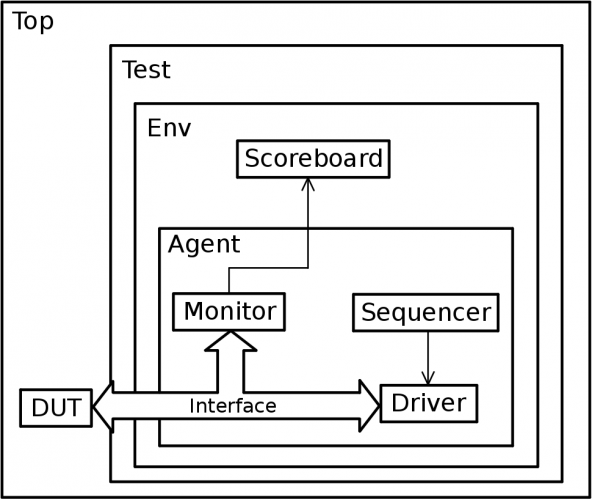
\includegraphics[width=0.35\textwidth]{uvm-tb_Pedro-Araujo.png}
    \caption{Representation of a simple UVM testbench. By Pedro Araújo / colorlesscube.com}
    \label{fig:uvm_testbench}
\end{figure}

%\ducky{an alternative graphic might be a layered (think networking, eg, TCP/IP or OSI model) graphic}


The main components of a UVM testbench are as follows:
%\kasper{Is this necessary? I had a difficult time understanding why all of the different components were necessary at first, but people with more verification experience might find it too basic?}
%\ducky{I think what this really needs (if this is needed at all) is an example that explains how all the parts work together, and what role they play in a whole testbench. The general argument for this is separation of concerns - it's not a great fit for small-scale testbenches like a single ALU, but makes more sense when working with complex systems and protocol buses. In a sense, it makes hard things easier, and easy things unnecessarily cumbersome - so does not scale down gracefully.}
%\kasper{Good point. Perhaps referencing the "First Experiments" with UVM at this point would help? Definitely agree that we should include the fact that UVM is mostly for large-scale testbenches, and doesn't make sense for a small-scale test such as a simple ALU}

    A \textit{Sequence(r):} defines the order of transactions necessary for a given purpose, e.g., synchronization or reset sequence. The sequencer is responsible for transferring the transactions, defined by the sequence, to the driver.
    
    A \textit{Driver} converts transactions into pin-level signals and drives these signals onto the DUT.
    
    An \textit{Interface} is a SystemVerilog construct which allows the user to group related signals. A DUT may have several interfaces attached.
    The interface is used to avoid hooking directly into the DUT, making it easier to test multiple DUT versions.
    
    A \textit{Monitor} monitors all traffic on the interface, converting pin-level signals into transaction-level objects that can be operated on by other components, such as a coverage collector or scoreboard.
    
    An \textit{Agent} encapsulates monitor, sequencer and driver, setting configuration values. Agents may be set active or passive (with or without a driver and sequencer). An agent is useful when it is necessary to have multiple instances of the same components, e.g., when a 4-port network switch needs four identical drivers with different configurations.
    
    A \textit{Scoreboard} is used to check whether correct functionality is achieved. Usually does so by using a ``golden model'' for co-simulation via the SystemVerilog direct programming Interface.
    
    The \textit{Environment} is used to configure and instantiate all child components. Environments are typically application-specific and may be modified by the test.
    
    The \textit{Test} is the top-level verification component. The test designer may choose to perform factory overrides of classes and set configuration values here, which modify the child components.

As shown above, even a ``Hello, World'' example using the UVM requires that the user understands how and why each of the different UVM components should be used. The use of so many components causes UVM to have a very steep learning curve, which may discourage adoption. This also means that UVM is not the proper testing methodology for small designs or one-off tests due to the initial workload.
However, once the initial setup of the testbench is finished for large and complex designs, generating new tests becomes easier.

%\martin{Does BluseSpec Verilog has something to offer?}
%\ducky{BSV is a higher-level design abstraction around guarded atomic actions - so relevant in terms of raising the level of design for digital logic, but a different approach than Chisel. My understanding (which may be outdated / wrong) is that BSV is propreitary, which is one reason it does not have significant traction. Earlier versions were heavily Haskell-based, which also does not help with perceived usability, supposedly that is why they're now branded "Bluespec SystemVerilog".}

\section{Open-Source Tools}
\label{sec:tools}

Our project plans to use mainly open-source tools, as we believe that only the open-source
movement can lead to tools for agile hardware development and open libraries for IPs
and verification components.

\subsection{Chisel}

Chisel is a hardware construction language embedded in Scala~\cite{chisel:dac2012}.
Chisel allows the user to write hardware generators in Scala, an object-oriented and functional language. For hardware generation and testing, the full Scala language and Scala and Java
libraries are available.
For example, we read in the string based schedules for a network-on-chip
%\footnote{available at: \url{https://github.com/t-crest/s4noc/tree/master/noc/vhdl/generated}}
and convert them with a few lines of Scala code into a hardware table to
drive the multiplexer of the router and the network interface.

\kasper{I don't quite understand this one - I don't see any Scala code in the directory. Is it the Java code in noc/src ?}
\martin{Maybe I should drop this, as the Scala code is in a different repo.}

Chisel is solely a hardware \emph{construction} language, and thus all valid Chisel code
maps to synthesizable hardware.
By separating the hardware construction and hardware verification languages,
it becomes impossible to write non-synthesizable hardware and in turn, speeds up the design process.
As Scala and Java's full power is available to the verification engineer,
the verification process is also made more efficient.


\martin{This is just a starting point, way more is needed.}
\kasper{Maybe take some of the points from the Introduction and move them here? We don't have that much space though, so I think it's fine.}

\subsection{ChiselTest}

While Chisel ultimately produces Verilog, which can be tested with industry-standard tools and processes, those generally force the user to pick between simple but limited (e.g., Verilog testbenches) or complex but powerful (e.g., UVM testbenches).

ChiselTest~\cite{chisel:tester2}, a nonsynthesizable testing framework for Chisel, instead emphasizes on usability and simplicity while providing ways to scale up complexity.

Fundamentally, ChiselTest is a Scala library that provides access into the simulator through operations like poke (write value into circuit), peek (read value from circuit, into the test framework), and step (advance time).
As such, tests written in ChiselTest are just Scala programs, imperative code that runs one line after the next.
This structure uses the latest programming language developments that have been implemented into Scala and provides a clean and concise interface, unlike approaches that attempt to reinvent the wheel like UVM.

Furthermore, ChiselTest tries to enable testing best practices from software engineering.
Its lightweight syntax encourages writing targeted unit tests by making small tests easy.
Furthermore, a clear and clean test code also enables the test-as-documentation pattern,
demonstrating a module's behavior from a temporal perspective.


\subsection{Simulators}

While Chisel designs can be simulated with any simulator that accepts Verilog input, there are trade-offs involved in choosing simulators.
Commercial simulators require expensive licenses, while the open-source Verilator has a high time cost for compilation despite being efficient per-cycle.
On the other hand, Treadle\footnote{\url{https://github.com/freechipsproject/treadle}} is a simulator that operates at the level of Chisel's intermediate representation, FIRRTL\footnote{\url{https://github.com/freechipsproject/firrtl}}.
Simulators like Treadle avoid the step of generating Verilog code and compiling from Verilog, which can vastly reduce the setup time for tests and efficiently run suites of many short tests.

Verilator has the benefit of compiling the Verilog code before simulating it. This is much faster compared to event-driven simulators but also limits the capabilites, as it only works on synchronous designs. Verilator claims to be on par or faster than the "Big 3" simulators on single thread. However, it also supports multi-threaded simulation, which can greatly improve simulation times for large designs \cite{verilator}.

\martin{Maybe a few words from Richard on Treadle, Simon on Verilator?}


\subsection{Scala}

The test environment and the driving code is written in Scala. Scala, with its
compatibility with Java, has a very rich open-source library ecosystem.
If you need a tool, e.g., an ELF file reader to load a binary, there will be a Java
library available for it.

Furthermore, we can use all the testing libraries that have been developed for
software development. A popular library is ScalaTest.\footnote{\url{https://www.scalatest.org/}}
A Chisel tester can be embedded
in a ScalaTest component, and a simple \code{sbt test} will execute all the tests.

\todo{Check what ScalaCheck can offer.}

\section{Integrating Legacy Languages}
\label{sec:legacy}

\kasper{I tried to polish this section as I felt it was a bit clunky. The original version is commented out below}
\begin{comment}
A verification method is only usable when it can handle mixed-source designs.
This means a Scala driven method must be able to test components written in Verilog,
VHDL, and SystemVerilog.

Chisel has support for black boxes, which allows the use of Verilog code within the Chisel design.
Therefore, it is relatively easy to integrate Verilog components when wrapped into a black box.
However, this forces Chisel to use Verilator instead of Treadle to run the simulation.

Chisel does not not fully support VHDL. It can support VHDL using VCS, but there is no
open-source solution available for VHDL.
However, VHDL is now a concern to companies that have a lot of source code written in VHDL, which needs to be compatible with any systems written in Chisel.
As many simulation and synthesis tools support mixed-language implementations,
this is not an issue for the implementation part. But for open-source testing, it proves to be a problem.

\martin{Simon, can you please update the description to what you have now?}

A solution for this is based on the principle of using synthesis tools to analyze the VHDL RTL code and synthesize a behavioral description for the component.
These synthesis tools can often output a Verilog-based netlist.
A free solution for this would be the Yosys \cite{Yosys} synthesis suite, which is an open-source digital hardware synthesis suite for Verilog code.
Yosys has support for VHDL by using Verific as a front-end, which requires a license.
For an alternative solution, we can use GHDL \cite{ghdl}.
GHDL is an open source simulator for VHDL that can also be used as a plugin for Yosys.
This allows Yosys to analyze VHDL files using GHDL and then synthesize a circuit.
The gate-level netlist can then be saved as a Verilog file, which can be used for the simulation system.
GHDL has full support for IEEE 1076 VHDL 1987, 1993, 2002 and a subset of 2008.
Thus, by using Yosys together with GHDL, it is possible to transpile VHDL to Verilog and then use a BlackBox to instantiate the generated Verilog code. This allows for an entirely open-source simulation toolchain no matter the HDL originally used.

\end{comment}

A verification method is only usable when it can handle mixed-source designs.
This means a Scala driven method must be able to test components written in Verilog,
VHDL, and SystemVerilog.

Chisel has support for black boxes, which allows the use of Verilog code within the Chisel design.
Therefore, it is relatively easy to integrate Verilog components when wrapped into a black box.
However, this forces Chisel to use Verilator instead of Treadle to run the simulation, impacting
startup time.

Chisel does not fully support VHDL. It can support VHDL using VCS, but there is no
open-source solution available for VHDL simulation. For companies with a lot of source code written in VHDL this is a concern, as they must be able to integrate their existing IP in a Scala/Chisel based design and verification workflow.
All major commercial simulation and synthesis tools support mixed-language designs, but no open-source tools exist that provide the same functionality.

\simon{Refs for Yosys and GHDL are missing}

\martin{Simon, the latest version does not really use a gate list, but something other. Can you elaborate?}
\kasper{From what you showed on Tuesday, it seems that Yosys/GHDL doesn't use the gate-level implementation, but works at the RTL level}

To alleviate this issue, the open-source Yosys synthesis suite \cite{Yosys} can be used. Yosys is an open-source digital hardware synthesis suite for Verilog. Yosys also has a variety of plugins, one of these being a plugin for using GHDL \cite{ghdl}, an open-source VHDL simulator. By using Yosys in conjunction with GHDL, VHDL files are compiled to an RTL-based intermediate representation, which is then written to a Verilog file using Yosys. GHDL has full support for IEEE 1076 VHDL 1987, 1993, 2002, and a subset of 2008. The workflow can be seen in Figure \ref{fig:VHDL2Verilog}. A working solution named VHDL2Verilog has been made for this, which has been tested with certain simple VHDL designs \cite{vhdl2verilog}.

\begin{figure}
    \centering
    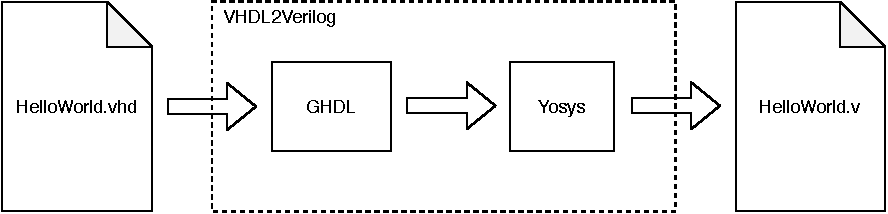
\includegraphics[width=\columnwidth]{VHDL2Verilog.pdf}
    \caption{VHDL2Verilog workflow}
    \label{fig:VHDL2Verilog}
\end{figure}

Thus, using Yosys together with GHDL, it is possible to transpile VHDL to Verilog and then use a BlackBox to instantiate the generated Verilog code. This allows for an entirely open-source simulation toolchain, no matter which HDL has been initially used.



\section{First Experiments}
\label{sec:eval}


Although this is a work-in-progress report, we have started with an evaluation.
We used an ALU with an accumulator from the Leros processor~\cite{leros:arcs2019}
as our device-under-test (DUT).
The example is simple, but has a combinational part and state in a register, being
a non-trivial circuit for testing.

The original design is in Chisel, and we reimplemented it in VHDL.
We wrote tests in SystemVerilog/UVM and Scala.
As execution platform, we used Synopsys VCS, ModelSim, Treadle, and Verilator.

We performed two experiments: (1) how to use hardware described in Chisel and VHDL in a
UVM test setup and (2) how to test Verilog and VHDL components in a Chisel/Scala
test setup.

\martin{We should have implementations in all languages we consider.}


\subsection{Using UVM with Chisel}

The Chisel toolchain translates Chisel code into plain Verilog for simulation and synthesis. Therefore, we can use a UVM based test bench to test Chisel generated code.
An important issue is that the modules and port names in the generated Verilog code are reasonable and do not change when changing the Chisel design.

We designed a UVM testbench to test the reference design's various implementations, the simple ALU from the Leros project.
Constrained-random verification is performed by generating random stimulus and edge-case stimuli, and functional coverage is collected. Also, we use a scoreboard to verify the functionality of the DUT. We describe the reference model in SystemVerilog.

As a SystemVerilog interface connects the DUT to the testbench, no details about the DUT are exposed to the driver and monitor. This makes it easy to replace the DUT with an alternative implementation, e.g., in another HDL, and verify its functionality. It is only necessary to instantiate the new DUT and connect it to the interface, after which the test can be run.

We run the UVM testbench on the Verilog description generated by Chisel and on a VHDL version of the ALU. Using the VHDL version required more manual work to make the mixed-language simulation work, whereas the Verilog version was very fast to implement. Generating Verilog with Chisel and testing with UVM then proves to be a suitable workflow. However, no open-source SystemVerilog simulator with UVM support is known.
Verilator primarily supports synthesizable constructs and does not support UVM, though this is on their roadmap~\cite{Snyder2019}.


\subsection{Mixed Language Verification with Chisel}
\label{sec:verif-chisel}

The initial experiment was to use UVM and test the VHDL and Chisel version of the
design. From Chisel code, we can generate Verilog, which we can test with UVM.
VCS and ModelSim support mixed language simulation (SystemVerilog and VHDL,
but not Chisel). Therefore, this was straight forward.

However, for the open-source tool-flow, we start from the Chisel implementation.
We wrote a test in Scala generating constraint-random values and comparing
the DUT output with the output of a simulation written in Scala. 
The Chisel/Sala version can execute in Treadle for  quick startup time or in Verilator
for higher performance.

A Verilog implementation can be used in the Chisel setup by wrapping the DUT
into a so-called \code{BlackBox}. When mixing Chisel with Verilog code, we need
to use Verilator as a simulation engine.
To reuse that Scala test with our VHDL implementation of the DUT, we use VHDL2Verilog
to convert the VHDL version of the DUT to Verilog and wrap it into a BlackBox.

To reuse the test for two different implementations, we use the object-oriented features
of Chisel/Scala. We define an abstract base class and extend that class by the Chisel
implementation and the Chisel wrapper for the Verilog implementation.
The tester expects the abstract base class.
Using object-oriented programming to describe hardware is an exclusive
feature of Chisel. SystemVerilog classes can only be used for test code,
not to describe hardware.

In the end, we have a setup where we can use the full power of Scala (and Java)
to test, co-simulate, and verify digital circuits described in Chisel, Verilog, or VHDL.
This setup consists of open-source tools only.

%\ducky{Likely criticism from peer review is that the example is too simple.}
%\ducky{I'd also like to see some kind of human evaluation - though I'm not sure what kind of methodology is accepted in the digital design community. Could maybe drop a HCI paper cite to hint that whatever methodology used is accepted in other communities.}

%\martin{We could also use my NoC example, which is not trivial ;-)}




\subsection{The Road Ahead}

\todo{ScalaTest and PBT with ScalaCheck.}

This work-in-progress paper is a first sketch of the ideas to combine SystemVerilog/UVM
with Chisel/Scala for a productive design and verification of future digital circuits.
We will explore all combinations with a few more examples, provided by our industrial
partners.
From that, we will bootstrap adding constraint-random verification methods to Chisel
testers and collecting coverage metrics within FIRRTL.

\subsection{Source Access}

As the project explores open-source tools for digital circuits design
and verification, we provide all examples, including this paper, in open-source
on GitHub:\\ \url{https://github.com/chisel-uvm}.


\section{Conclusion}
\label{sec:conclusion}

This work-in-progress paper is a first sketch of the ideas to combine SystemVerilog/UVM
with Chisel/Scala for a productive design and verification of future digital circuits.
We will explore all combinations with examples provided by our industrial partners.



\subsection*{Acknowledgment}

This work has been performed as part of the
``InfinIT -- Innovationsnetv{\ae}rk for IT'', UFM case no. 1363-00036B,
``High-Level Design and Verification of Digital Systems''.


%This work was partially funded under the
%European Union's 7th Framework Programme
%under grant agreement no. 288008:
%Time-predictable Multi-Core Architecture for Embedded
%Systems (\mbox{T-CREST}).

%\newpage


\bibliographystyle{plain}
% Please do not add any references to msbib.bib.
% They get lost when I 'generate' is again (see Makefile)
\bibliography{chisel-uvm,msbib}

\end{document}
~
\newpage
~
\newpage

\section{The Classic Hardware Description Languages}

\section{SystemVerilog}

\todo{adds some VHDL features to Verilog. Tries to please VHDL developers.}

SystemVerilog is IEEE standard, proprietary tools.

Chisel is research stuff and open-source

\section{Chisel}

Chisel~\cite{chisel:dac2012} 

\section{Combining the Approaches}

Although SystemVerilog/UVM and Chisel/Scala look like competing initiatives
to solve the verification problem, it should be possible to combine those two methods.
By using this combination we might be able to enjoy the benefits of both worlds:
the industrial proven SystemVerilog/UVM tool chain with the available IPs with
the research and more software oriented approach of Chisel/Scala. 

\todo{Be nice to all and show how we can combine different approach to
get the best of both worlds}

\ducky{The main nontechnical benefits of UVM are a large library and userbase, and this inertia is probably going to hamper adoption of a new tool, especially if that new tool is more incremental than revolutionary. To my understanding, the main technical benefits of UVM are re-use and separation of responsibilities, and is inspired by an old-ish (and fairly verbose) form of OO}

\subsection{Using UVM with Chisel}

The Chisel toolchain translates Chisel code into plain Verilog for simulation and
synthesis. Therefore, we can use a UVM based test bench to test Chisel generated code.
An important issue is that the modules and port names in the generated Verilog
code are reasonable and do not change when changing the Chisel design.

\subsection{UVM with VHDL}
\kasper{Shouldn't this actually be UVM with (System)Verilog? Or are we focusing specifically on VHDL because UVM isn't made for VHDL, and thus we're looking into what's possible?}
\martin{One can also use UVM/SystemVerilog test logic with a VHDL DUT.}

\subsection{Chisel with Verilog}

\subsection{Chisel with VHDL}

\subsection{Chisel with UVM}

\todo{reusing Chisel tests (ScalaTest) within the UVM framework
with the generated Verilog code}
\ducky{UVM is largely a framework and library for testing blocks ("IP"), I don't think transpiling ChiselTest to UVM is feasible. Best I would practically hope for is interop between both, eg ChiselTest hooks to call UVM functions in a Verilog simulation environment, to enable continued use of legacy test code, Not sure the other way around is worth doing (calling ChiselTest functions from within a UVM environment)}

\section{Co-Simulation}

\todo{with C/C++/Java/Scala/Phyton, ....}
\ducky{Should be tons of this already. CoCoTb is a Python cosimulation environment. Rocket-chip uses C++ cosimulation in their RTL tests.}


\section{Notes}

Here collect of notes and ideas in bullet list for the development and writing process:

\begin{itemize}
\item Collect related work
\item Some more notes
\end{itemize}

\subsection{Comparison}

\begin{itemize}
\item UVM is directly supported in major tools
\item UVM is based on SystemVerilog (SV)
\item OO in SV is only for test benches, not for HW description
\item SystemVerilog is three languages in one: old Verilog, new SystemVerilog for synthesize
(what constructs are supported by what tool), and SV for test benches
\item SV is a specialized language for HW design and testing
\item Chisel is two languages: Chisel for HW and Scala for tester
\item Chisel supports OO for HW description
\item Chisel is based on Scala
\item Scala is a general purpose languages
\item Scala/Chisel can use Java libraries (a LOT is available)
\item Number of Scala programmers are larger than SV programmers (how much?)
\item UVM is open source
\item SV implementation is closed source, needs commercial tools
\item UVM/SV is available on EDAPlayground
\item Chisel/Scala is open source
\item Chisel/Scala runs on the JVM, on Windows, Linux, and macOS
\item Chisel is missing the UVM methodology
\item SV (tools) supports coverage, Chisel does not
\item UVM provides functions for random constraint testing, Chisel/Scala not
\item UVM has a lot of IPs available (e.g., AXI)
\item Chisel testers need some library for sequencing and interfacing (bachelor/master thesis on parts)
\item Verdi is a GUI with knowledge of UVM
\item Verilator with C/C++ emulation is another verification option
\item SV has 250 keywords!
\item The spec of SV does not define what subset is sythesisable, see also \url{https://sutherland-hdl.com/papers/2013-SNUG-SV_Synthesizable-SystemVerilog_presentation.pdf}
\item From a chat at FPL: ``He said ``every day'', so I assumed he could help me with the most complex features of SV! Turns out they write all their synthesis code in the lowest level RTL possible, down to the bit, and just use SV for a couple of language constructs in testbenches here and there (like structs and typedefs). Nothing that couldn't be accomplished without SV, by his admission. When you consider the size of the SV standard, I'm not so sure that SV is ``used'' in industry in its true sense.''
\item Another from that chat: ``Different tools supported different subsets of SV for synthesis, but they didn't tend to publish this list. As you say, we had to check *everything* first.''
\end{itemize}

\subsection{Research Questions}

\begin{itemize}
\item Can we use Chisel testers within UVM?
\item Can we run JVM based code in UVM?
\item Doing UVM verification on Chisel generated Verilog
\item UVM testing on Chisel interpreter (like Chisel tester using treadle, or Verilator)
\end{itemize}

\subsection{Big Research Questions}

These topics are probably good questions for a larger research project.
Part of this is probably already looked at by PhD students at UCB.

\begin{itemize}
\item Add coverage to Chisel tester
\item Provide random constraint functions
\item Provide UVM functions
\item 
\item 
\end{itemize}

\subsection{Helpful links and resources}

VHDL/SV comparison: \url{http://www.sunburst-design.com/papers/CummingsSNUG2003Boston_SystemVerilog_VHDL.pdf}

Open-source design flow, maybe for the Basys3: \url{https://symbiflow.github.io/}

Video primer on using UVM, explains what each component of the UVM test does and why things are set up the way they are
\url{https://www.youtube.com/watch?v=FkclDiK4Oco}

Website that has relatively in-depth and understandable explanations of UVM concepts and structure
\url{https://www.chipverify.com/uvm/uvm-hello-world}






\end{document}

%% Adding a comment to test linking with overleaf
